\documentclass[12pt,a4paper]{article}
\usepackage[utf8]{inputenc}
\usepackage[francais]{babel}
\usepackage{amsmath}
\usepackage{amsfonts}
\usepackage{amssymb}
\usepackage{stmaryrd}
\usepackage{float}
\usepackage{systeme}
\setlength{\oddsidemargin}{-18pt}
\setlength{\evensidemargin}{-18pt}
\setlength{\textwidth}{481pt}
\setlength{\textheight}{710pt}
\setlength{\headheight}{-53pt}
\setlength{\footskip}{18pt}
\usepackage[hyperindex]{hyperref}
\newtheorem{dfn}{\textbf{Définition}}[subsection]
\newtheorem{thm}[dfn]{\textbf{Théoreme}}
\newtheorem{prop}[dfn]{\textbf{Proposition}}
\newtheorem{cor}[dfn]{\textbf{Corollaire}}
\newtheorem{lem}[dfn]{\textbf{Lemme}}
\usepackage[nothm]{thmbox}

\usepackage{graphicx}
\usepackage{caption}

\newcommand{\rot}{\text{rot}}

\numberwithin{equation}{section}
\def\proof{\begin{thmbox}[M]{\textbf{Preuve :}}}
\def\endproof{\end{thmbox}}
\begin{document}
\title{Analyse spectrale d'écoulements fluides et modèles d'amortissement}
\author{Lesage Adrien}
\maketitle
\newpage
\tableofcontents
\newpage
\section{Introduction aux équations d'Euler à surface libre.}
\subsection{Hypothèses}

Tout le long de ce mémoire, nous nous intéresserons à l'étude d'un fluide dont nous supposerons les hypothèses suivantes vérifiées
\begin{list}{}{}
    \item[$(\textbf{H}_1)$ : ] Le fluide est \textit{homogène} et \textit{incompressible}.
    \item[$(\textbf{H}_2)$ : ] Le fluide est \textit{non visqueux}.
    \item[$(\textbf{H}_3)$ : ] Le fluide est \textit{irrotationnel}.
\end{list}

Soit $\textbf{X} = \mathbb{R}^d$ avec $d \in \{1,2\}$. On souhaite étudier un tel fluide évoluant dans le domaine $$\Omega_t = \left\{ (x,z) \in \textbf{X}\times\mathbb{R}  \,|\quad b(x) - H_0 \leq z \leq \zeta(t,x) \,\right\}$$
\begin{list}{}{}
\item[\textbullet] $b : \textbf{X}\rightarrow \mathbb{R}$ désigne les variations du fond du fluide, de profondeur caractéristique $H_0 > 0$
\item[\textbullet] le graphe $\zeta : \mathbb{R}_+\times \textbf{X}$ désigne la surface du fluide, de sorte que les hypothèses suivante soient vérifiées
\end{list}
\begin{list}{}{}
    \item[$(\textbf{H}_4)$ : ] Les particules de fluide ne traversent pas le fond.
    \item[$(\textbf{H}_5)$ : ] Les particules de fluide ne traversent pas la surface.
    \item[$(\textbf{H}_6)$ : ]  En tout point $x\in\textbf{X}$ et en tout instant $t\geq 0$, l'épaisseur du fluide $\zeta(t,x) - (b(x)-H_0)$ est supérieure à une constante $H_0>0$ indépendante de $x$ et de $t$.
    \item[$(\textbf{H}_7)$ : ] La pression  du fluide à la surface est égale à la pression atmosphérique $P_{\text{atm}}$ (on néglige les tensions de surface).
    \item[$(\textbf{H}_8)$ : ] Le fluide est soumis à une force de gravité d'intensité $g$ et de direction opposée au vecteur $\textbf{z} = (0_{\textbf{X}},1)$.
    \item[$(\textbf{H}_9)$ : ] Le fluide est au repos à l'infini et $\lim\limits_{\|x\|\rightarrow \infty}\zeta(x,t) = 0$
\end{list}

\begin{center}
    \texttt{ajouter schéma}
\end{center}


\subsection{Formulation des équations d'Euler.}
\subsubsection{Formulation de l'évolution du champ de vitesse}
Pour commencer, nous allons adopter un point de vue lagrangien:
\begin{list}{}{}
    \item[\textbullet] Posons $\left(\begin{array}{l}
         \mathcal{X}\\
         \mathcal{Z}
    \end{array}\right) :  \mathbb{R}_+ \rightarrow \textbf{X}\times\mathbb{R}$ la fonction qui suit le déplacement d'une particule de fluide de position initiale $\left(\begin{array}{l}
         \mathcal{X}\\
         \mathcal{Z}
    \end{array}\right)(0)  \in \Omega_0$.
    \item[\textbullet] Posons $\textbf{U}(t,x,z)$ la vitesse d'une particule de fluide située en $(x,z) \in \Omega_t$ à l'instant $t$.
\end{list}
Les hypothèses $(\textbf{H}_4)$ et $(\textbf{H}_5)$ nous donnent que $\left(\begin{array}{l}
         \mathcal{X}\\
         \mathcal{Z}
\end{array}\right)\in \Omega_t$ pour tout instant $t \geq 0$. Ceci nous permet d'écrire
    
\begin{equation}
\frac{d}{dt} \left(\begin{array}{l}
         \mathcal{X}\\
         \mathcal{Z}
\end{array}\right) = U(t,\mathcal{X}(t), \mathcal{Z}(t)) 
\end{equation}

En dérivant une fois de plus, on obtient 
$$
\frac{d^2 }{dt^2}\left(\begin{array}{l}
         \mathcal{X}\\
         \mathcal{Z}
\end{array}\right)  = \frac{\partial \textbf{U}(t,\mathcal{X}(t),\mathcal{Z}(t))}{\partial t} + \text{Jac}(\textbf{U})\frac{d}{d t}\left(\begin{array}{l}
         \mathcal{X}\\
         \mathcal{Z}
\end{array}\right) 
$$
    Ou, autrement dit,
    
$$
\frac{d^2 }{dt^2}\left(\begin{array}{l}
         \mathcal{X}\\
         \mathcal{Z}
\end{array}\right)= \left(\frac{\partial\textbf{ U}}{\partial t}+ (\textbf{U}\cdot \nabla ) \textbf{U}\right)(t,\mathcal{X}(t),\mathcal{Z}(t)) 
$$

Les hypothèses $(\textbf{H}_2)$ nous dit que les particules ne s'influencent pas mutuellement en dehors de la pression. Chaque particule n'est alors soumis qu'à deux forces: la force de gravité $ F_\text{g} = -\rho g\textbf{z}$ et la force de pression $F_\text{P} = - \nabla\textbf{P}$. La deuxième loi de Newton donne alors

$$
\rho\frac{d^2 }{dt^2}\left(\begin{array}{l}
         \mathcal{X}\\
         \mathcal{Z}
\end{array}\right)(t) = - \rho g \textbf{z} -\nabla P(t,X(t),\mathcal{Z}(t))
$$
Ce qui nous donne les équations d'Euler définies par le système suivant.

\begin{equation} 
\tag{$\textbf{E}_1$} \label{eq_E1}
\rho \left( \frac{\partial U}{\partial t} + (\textbf{U}\cdot \nabla ) \textbf{U} \right) + \rho g\textbf{z} + \nabla \textbf{P} = 0
\end{equation}


\subsubsection{Formulation de la condition d'incompressibilité}
L'hypothèse $(\textbf{H}_1)$ se traduit par
$$\rho(t,x,z) = \rho_0$$
En conséquence, la loi de conservation de la masse d'un fluide
\begin{equation} \label{mass_conservation}
    \frac{\partial \rho}{\partial t} - \text{div}(\rho\textbf{U}) = 0
\end{equation}
devient
\begin{equation} \tag{$\textbf{E}_2$} \label{divergence_free}
    \text{div} (\textbf{U}) = 0
\end{equation}

\subsubsection{Formulation des conditions aux bords et de l'évolution de la surface}

L'hypothèse $(\textbf{H}_4)$ s'exprime ainsi

\begin{equation}
    \tag{${\textbf{E}}_3$} \label{eq_E2}
    \textbf{U}.\textbf{n} = 0 \text{  sur }\{z = b(x)-H_0\}
\end{equation} 

où \textbf{n} désigne le vecteur normal extérieur au domaine $\Omega_t$.\\

Cette formule est une réécriture immédiate $(\textbf{H}_4)$  car $b-H_0$ ne dépend pas du temps. En revanche, comme $\zeta$ dépend du temps, la caractérisation de l'hypothèse $(\textbf{H}_5)$ est moins immédiate et est l'objet de la proposition suivante.



\begin{prop} L'hypothèse $(\textbf{H}_5)$ nous donne que
    \begin{equation} \tag{$\textbf{E}_4$} \label{eq_E3}
        \frac{\partial \zeta}{\partial t}(t,x) - \sqrt{1+ \| \nabla_\textbf{X}\zeta\|^2} \textbf{U} \cdot \textbf{n} = 0 \quad\text{dans}\,\{z = \zeta(t,x)\}
    \end{equation}
    où $\textbf{n}$ désigne le vecteur normal extérieur au domaine $\Omega_t$
\end{prop}
\begin{proof}
\textit{Etape 1 : }Commençons par déterminer $\textbf{n}$ en fonction de $t$, $x$, et $\zeta$. A $t$ fixé, la surface est paramétrée par l'application $$S_t: x\in \textbf{X} \mapsto \left(\begin{array}{l}
         x\\
         \zeta(t,x)
    \end{array}\right).$$
Sa différentielle en $x$ est 
$$DS_t(x) : v \in \textbf{X} \mapsto DS_t(x).v = \left(\begin{array}{l}
         v\\
         \nabla_X\zeta(t,x) \cdot v
    \end{array}\right).$$
Le vecteur normal \textbf{n} vérifie alors $$\textbf{n}\cdot (DS_t(x).v) = 0$$
pour tout $v \in \textbf{X}$. En posant $\textbf{n} = \left(\begin{array}{l}
         n_1\\
         n_2
    \end{array}\right)$, on trouve alors
    $$ \left(n_1 + n_2\nabla_X\zeta(t,x)\right)\cdot v = 0$$
pour tout $v\in\textbf{X}$. On a alors
$$ n_1 =  - n_2\nabla_X\zeta(t,x)$$
Donc $\textbf{n} = n_2\left(\begin{array}{l}
         - \nabla_X\zeta(t,x)\\
         1
    \end{array}\right)$
Comme la normale est dirigée vers le haut, il vient que $n_2>0$ et comme $\|\textbf{n}\| = 1$, on trouve finalement \begin{equation} \label{normal_surface_vector}
\textbf{n} = \frac{1}{\sqrt{1+\|\nabla_X\zeta(t,x)\|^2}}\left(\begin{array}{l}
         - \nabla_X\zeta(t,x)\\
         1
    \end{array}\right)\end{equation}
\textit{Etape 2 : }Considérons à nouveau $\left(\begin{array}{l}
         \mathcal{X}\\
         \mathcal{Z}
\end{array}\right)$ 
la trajectoire d'une particule et supposons qu'elle est initialement située à la surface. l'hypothèse nous donne qu'alors la particule ne peut traverser la surface ni dans un sens, ni dans l'autre. Il y a alors, pour tout temps $t \geq 0$, l'égalité suivante.
$$\mathcal{Z} - \zeta( . ,\mathcal{X}) = 0 $$
En dérivant cette égalité, il vient
\begin{align*} 
    0 &= \frac{d\mathcal{Z}}{dt} - \frac{\partial \zeta}{\partial t}(.,\mathcal{X}) - \nabla_\textbf{X}\zeta(.,\mathcal{X}) \cdot \frac{d \mathcal{X}}{dt} \\ 
    &=  \textbf{U}\cdot  \left(\begin{array}{l}
         - \nabla_X\zeta(t,x)\\
         1
    \end{array}\right) - \frac{\partial \zeta}{\partial t}(.,\mathcal{X}) 
    \\&= \sqrt{1 + \|\zeta\|^2}\textbf{U}  \cdot \textbf{n} - \frac{\partial \zeta}{\partial t}(.,\mathcal{X}) 
\end{align*}



\end{proof}

\paragraph{Pour résumer,} en combinant (\ref{eq_E1}), (\ref{divergence_free}), (\ref{eq_E2}) et (\ref{eq_E3}), on obtient les équations d'Euler à surface libre
\begin{equation} \tag{\textbf{E}}
    \left\{ 
    \begin{aligned}
        &\rho \left ( \frac{\partial \textbf{U}}{\partial t} + (\textbf{U}\cdot \nabla ) \textbf{U}+  g\textbf{z}  \right) + \nabla \textbf{P} = 0 & &  
        \\
        &\text{div}(\textbf{U}) = 0 & &  
        \\
        &\textbf{U}.\textbf{n} = 0 &\text{dans}\,\{z = b(x)-H_0\}& 
        \\
        &\frac{\partial \zeta}{\partial t}(t,x) - \sqrt{1+ \| \nabla_\textbf{X}\zeta\|^2} \textbf{U} \cdot \textbf{n} = 0 &\text{dans}\,\{z = \zeta(t,x)\} & 
    \end{aligned}
    \right.
\end{equation}
\paragraph{Remarque :} L'égalité vectorielle suivante
$$(\textbf{U}\cdot \nabla ) \textbf{U} = \rot(\textbf{U})\wedge \textbf{U} + \frac{1}{2}\nabla |\textbf{U}|^2$$
Nous permet de réécrire (\ref{eq_E1}) sous la forme
\begin{equation} \label{eq_E1bis}
    \rho \left( \frac{\partial \textbf{U}}{\partial t} +\rot(\textbf{U})\wedge \textbf{U} + \frac{1}{2}\nabla |\textbf{U}|^2+  g\textbf{z}  \right) + \nabla \textbf{P} = 0 
\end{equation}

Ainsi, l'hypothèse $(\textbf{H}_3)$, qui se traduit par $\rot(\textbf{U})=0$, permet alors d'avoir 
\begin{equation} \tag{$\textbf{E}_{1,\text{bis}}$} \label{eq_E1bis}
        \rho \left( \frac{\partial \textbf{U}}{\partial t} +\frac{1}{2}\nabla  |\textbf{U}|^2 +  g\textbf{z}\right) + \nabla \textbf{P} = 0 
\end{equation}

\subsection{Formulation de Bernoulli}

Grace notament à $(\textbf{H}_6)$, on sait que $\Omega_t$ est simplement connexe à tout instant $t$, et comme $\rot(\textbf{U}) = 0$, on en déduit alors l'existence d'une fonction $\Phi(t,.,.): \textbf{X}\times \mathbb{R} \rightarrow \mathbb{R}$ telle que $$\textbf{U} = \nabla \phi  \;.$$    

Ceci permet de réécrire le système (\ref{eq_E1bis}).

\begin{align*}
    0 = &\rho \left ( \frac{\partial \nabla \phi }{\partial t} +\frac{1}{2}\nabla  |\nabla \phi|^2  +  g\textbf{z} \right)+ \nabla \textbf{P} 
    \\
    =&\nabla \left ( \rho \left ( \frac{\partial \phi }{\partial t} +\frac{1}{2}|\nabla \phi|^2 +  gz \right) + \textbf{P} \right)
    \\
    =&\nabla \left ( \rho \left ( \frac{\partial \phi }{\partial t} +\frac{1}{2}|\nabla \phi|^2 +  gz \right) + \textbf{P}  - \textbf{P}_{\text{atm}}\right)
\end{align*}

Une condition suffisante pour verifier (\ref{eq_E1bis}) est alors
\begin{equation} \tag{$\textbf{B}_1$} \label{eq_B1}
  \frac{\partial \phi }{\partial t} +\frac{1}{2}|\nabla \phi|^2 +  gz   = \frac{1}{\rho}\left( \textbf{P}_{\text{atm}}  - \textbf{P}\right)
\end{equation}

Et comme $\text{div}(\nabla \phi) = \Delta \phi$, la condition d'incompressibilité (\ref{divergence_free}) devient alors

\begin{equation} \tag{$\textbf{B}_2$} \label{eq_B2}
    \Delta \phi = 0
\end{equation}

L'équation (\ref{eq_E2}), devient

\begin{equation} \tag{$\textbf{B}_3$} \label{eq_B3}
    \frac{\partial \phi}{\partial \textbf{n}} = 0 ~~~ \text{dans}\,\{z = b(x)-H_0\} .
\end{equation}

L'équation (\ref{eq_E3}), devient

\begin{equation} \tag{$\textbf{B}_4$} \label{eq_B4}
\frac{\partial \zeta}{\partial t}  - \sqrt{1+ \| \nabla_\textbf{X}\zeta\|^2}\frac{\partial \phi}{\partial\textbf{n}} = 0~~~\text{dans}\,\{z = \zeta(t,x)\} .
\end{equation}

Sachant (\ref{normal_surface_vector}), on connaît et on utilisera souvent l'équivalence entre (\ref{eq_B4}) et l'équation suivante


\begin{equation} \label{eq_B4_bis}
    \frac{\partial \zeta}{\partial t}  + \nabla_\textbf{X}\zeta\cdot\nabla_\textbf{X}\phi - \frac{\partial\phi}{\partial z} = 0 ~~~\text{dans}\{z = \zeta(t,x)\} 
\end{equation}

De manière analogue, on a aussi équivalence entre (\ref{eq_B3}) et 

\begin{equation} \label{eq_B3_bis}
    \nabla_\textbf{X}b\cdot\nabla_\textbf{X}\phi - \frac{\partial\phi}{\partial z} = 0 ~~~\text{dans}\{z = b(x)\} 
\end{equation}



\subsection{Formulation de Craig-Sulem-Zakharov}
\subsection{Adimensionnement des paramètres du système}

\begin{center}
    \texttt{ajouter schéma}
\end{center}

On va chercher à réécrire ces équations en faisant apparaître les rapports entre les différentes grandeurs caractéritiques qui entrent en jeux. Ainsi la négligeabilité d'un paramètre relativement à un autre s'impactera sur nos équation sous la forme d'une possible simplification de un ou plusieurs termes. Une équation ne faisant intervenir que des rapports adimmensionés est dites adimmensionelle. 
\\

Dans notre cas, les grandeurs caractéristiques de notre système sont

\begin{list}{\textbullet}{}
    \item $H_0$ est la profondeur du système.
    \item $a_{\text{surf}} = max(|\zeta|)$ est l'amplitude de la surface du fluide.
    \item $a_{\text{bot}} = max(|b|)$ est l'amplitude du fond du fluide.
    \item $L_1$ est la longueur d'onde de $\zeta$ dans la direction $\textbf{e}_1$.
    \item $L_2$ est la longueur d'onde de $\zeta$ dans la direction transversale $\textbf{e}_2$ (si $\textbf{X} = \mathbb{R}^2)$.
    
 \end{list}
\,
\\

On étudiera les rapports suivants.

\begin{list}{\textbullet}{}
    \item $\varepsilon = \frac{a_{\text{surf}}}{H_0}$ le coefficient de \textit{non-linéarité} du système.
    \item $\mu =\frac{H_0^2}{L_1^2}$ le coefficient de \textit{profondeur}.
    \item $\beta = \frac{a_{\text{bot}}}{H_0}$ est le coefficient de \textit{dénivellation} du fond.
    \item $\gamma = \frac{L_1}{L_2}$ est le coefficient de \textit{transversalité}.
    \item $\epsilon = \frac{ a_{\text{surf}}}{L_1}$ le coefficient d'\textit{amplitude}.
    \item $t_0 = \frac{L_1}{\sqrt{gH_0}}$ est l'échelle de temps caractéristique.
\end{list}

~\\
Pour adimensionner nos équations, on pose l'isomorphisme linéaire suivant:

  
\begin{equation}
\begin{aligned}
      \mathcal{I}:~~&\mathbb{R}\times\textbf{X}\times\mathbb{R} &\longrightarrow ~~~ &\textbf{X}\times \mathbb{R} & \\
      &(t,(x_1,x_2),z) &\longmapsto &\left(\frac{t}{t_0},\left(\frac{x_1}{L_1},\frac{x_2}{L_2} \right),\frac{z}{H_0}\right) ~~~&\text{si }\textbf{X}=\mathbb{R}^2\\
      &(t, x ,z) &\longmapsto &\left(\frac{t}{t_0},\frac{x}{L_1},\frac{z}{H_0}\right) ~~~&\text{si }   \textbf{X}=\mathbb{R}
\end{aligned}
\end{equation}

    
   
    


~\\

On effectue le changement de variable suivant.

\begin{list}{\textbullet}{}
    \item $(t',x',z') = \mathcal{I} (t,x,z)$
    \item $\zeta' = \dfrac{1}{a_{\text{surf}}}(\zeta \circ \mathcal{I}^{-1})$ 
    \item $b' = \dfrac{1}{a_{\text{bot}}}(b\circ\mathcal{I}^{-1})$
     \item $\phi' = \dfrac{1}{g t_0 a_{\text{surf}}}(\phi \circ \mathcal{I}^{-1})$
     \item $P' = \dfrac{t_0^2}{H_0^2\rho_0} (P \circ \mathcal{I}^{-1})~~~~~~~$   (et $P_{\text{atm}}' = \dfrac{t_0^2}{H_0\rho_0} P_\text{atm}$)
\end{list}

Ceci nous donne, entre autre, 
\begin{align}
    &-1 \leq \zeta' \leq 1\\ &-1 \leq b' \leq 1 
\end{align}
\subsubsection{Adimensionnement des équations de Bernoulli pour $\textbf{X} = \mathbb{R}$}
Pour $\textbf{X} = \mathbb{R}$, l'adimensionnement de (\ref{eq_B1}) s'éffectue ainsi:
\begin{align}
    \text{(\ref{eq_B1})} &\Leftrightarrow \frac{g t_0 a_{\text{surf}}}{t_0}\partial_{t'} \phi' + \frac{1}{2}\left(\frac{(g t_0 a_{\text{surf}})^2}{L_1^2}(\partial_{x'}\phi')^2+ \frac{(g t_0 a_{\text{surf}})^2}{H_0^2}(\partial_{z'}\phi')^2\right) + g H_0 z' = \frac{1}{\rho_0}\frac{H_0^2\rho_0}{t_0^2}(P'-P'_{\text{atm}}) \nonumber\\
    &\text{On factorise le terme non linéaire par $ \frac{(g t_0 a_{\text{surf}})^2 }{L_1^2}$ , ce qui fait apparaître $\mu$.}\nonumber\\
     &\Leftrightarrow  g  a_{\text{surf}} \partial_{t'} \phi' + (g t_0 a_{\text{surf}})^2\frac{1}{2L_1^2}\left( (\partial_{x'}\phi')^2+ \frac{1}{\mu}(\partial_{z'}\phi')^2\right) + g H_0 z' =  \frac{H_0^2  }{t_0^2}(P'-P'_{\text{atm}})\nonumber\\
     &\text{On développe $gt_0$ dans ce terme.}\nonumber\\
     &\Leftrightarrow  g  a_{\text{surf}} \partial_{t'} \phi' + 
     ( \sqrt{g}\frac{L_1}{\sqrt{H_0}} a_{\text{surf}})^2
     \frac{1}{2L_1^2}
     \left( (\partial_{x'}\phi')^2+ \frac{1}{\mu}(\partial_{z'}\phi')^2\right) 
     + g H_0 z' 
     = \frac{H_0^2 }{t_0^2}(P'-P'_{\text{atm}})\nonumber\\
     &\text{On simplifie ce terme.}\nonumber\\
    &\Leftrightarrow  g  a_{\text{surf}} \partial_{t'} \phi' + 
     \frac{g a_{\text{surf}}^2}{2H_0}
     \left( (\partial_{x'}\phi')^2+ \frac{1}{\mu}(\partial_{z'}\phi')^2\right) 
     + g H_0 z' 
     = \frac{H_0^2  }{t_0^2}(P'-P'_{\text{atm}})\nonumber\\
     &\text{On voit apparaître $\varepsilon$.}\nonumber\\
     &\Leftrightarrow  g  a_{\text{surf}} \partial_{t'} \phi' + 
     \varepsilon\frac{g a_{\text{surf}}}{2}
     \left( (\partial_{x'}\phi')^2+ \frac{1}{\mu}(\partial_{z'}\phi')^2\right) 
     + g H_0 z' 
     = \frac{H_0^2 }{t_0^2}(P'-P'_{\text{atm}})\nonumber\\
     &\text{On divise tout par $g  a_{\text{surf}}$ et on voit à nouveau apparaître $\varepsilon$ et $\mu$}. \nonumber\\
     &\Leftrightarrow   \partial_{t'} \phi' + 
     \frac{\varepsilon}{2}
     \left( (\partial_{x'}\phi')^2+ \frac{1}{\mu}(\partial_{z'}\phi')^2\right) 
     + \frac{z'}{\varepsilon} 
     = \frac{\mu}{\varepsilon}(P'-P'_{\text{atm}}) \label{eq_B1_adim}
\end{align}
\\

L'adimensionnement de (\ref{eq_B2}) s'effectue ainsi:
\begin{align}
    \text{(\ref{eq_B2})} &\Leftrightarrow  \frac{(g t_0 a_{\text{surf}})}{L_1^2}\partial_{x' x'}\phi'+ \frac{(g t_0 a_{\text{surf}})}{H_0^2}\partial_{z' z'}\phi'  = 0\nonumber\\
    &\text{On divise le tout par $ \frac{(g t_0 a_{\text{surf}})^2 }{H_0^2}$ , ce qui fait apparaître $\mu$.}\nonumber\\
    &\Leftrightarrow \partial_{z'z'}\phi' + \mu \partial_{x_1' x_1'}\phi'  = 0 \label{eq_B2_adim}
\end{align}

L'adimensionnement de (\ref{eq_B3}) s'effectue ainsi

\begin{align}
\text{(\ref{eq_B3})} &\Leftrightarrow \text{(\ref{eq_B3_bis})}& ~ \nonumber\\
&\Leftrightarrow \partial_x b \partial_x\phi - \partial_z\phi = 0 & \text{dans }\{z = b(x) - H_0\} \nonumber\\
&\Leftrightarrow \left(\frac{a_{\text{bot}}}{L_1} \partial_{x'} b'\right)\left(\frac{gt_0a_{\text{surf}}}{L_1}\partial_{x'}\phi'\right)  - \frac{gt_0a_{\text{surf}}}{H_0}\partial_{z'}\phi' = 0& \text{dans }\{z' = \beta b'(x') - 1\}\nonumber\\
&\Leftrightarrow  \frac{a_{\text{bot}}H_0}{L_1^2} \partial_{x'} b'  \partial_{x'}\phi'   - \partial_{z'}\phi' = 0& \text{dans }\{z' = \beta b'(x') - 1\}\nonumber\\
&\Leftrightarrow  \beta \mu \partial_{x'} b'  \partial_{x'}\phi'   - \partial_{z'}\phi' = 0& \text{dans }\{z' = \beta b'(x') - 1\}\label{eq_B3_adim}
\end{align}

L'adimensionnement de (\ref{eq_B4}) s'effectue ainsi

\begin{align}
\text{(\ref{eq_B4})} &\Leftrightarrow \text{(\ref{eq_B4_bis})}& ~ \nonumber\\
&\Leftrightarrow \partial_t\zeta + \partial_x \zeta \partial_x\phi - \partial_z\phi = 0 & \text{dans }\{z = \zeta(x,t)\} \nonumber\\
&\Leftrightarrow \frac{a_{\text{surf}}}{t_0}\partial_{t'} \zeta' + \left(\frac{a_{\text{surf}}}{L_1} \partial_{x'} \zeta '\right)\left(\frac{gt_0a_{\text{surf}}}{L_1}\partial_{x'}\phi'\right)  - \frac{gt_0a_{\text{surf}}}{H_0}\partial_{z'}\phi' = 0& \text{dans }\{z' = \varepsilon \zeta(t',x')\}\nonumber\\
&\Leftrightarrow \partial_{t'}\zeta' +  \frac{gt_0^2a_{\text{surf}}}{L_1^2} \partial_{x'} \zeta ' \partial_{x'}\phi'  - \frac{gt_0^2}{H_0}\partial_{z'}\phi' = 0&  \text{dans }\{z' = \varepsilon \zeta(t',x')\} \nonumber \\
&\Leftrightarrow \partial_{t'}\zeta' +  \varepsilon \partial_{x'} \zeta ' \partial_{x'}\phi'  - \frac{1}{\mu}\partial_{z'}\phi' = 0&  \text{dans }\{z' = \varepsilon \zeta(t',x')\} \label{eq_B4_adim}
\end{align}






Par la suite, lorsqu'on travaillera sur les équations adimensionnées, on se permettra d'omettre les apostrophes sur ces variables.
\newpage
\section{Cas du fond plat 1D} 

Dans cette partie on s'intéressera au cas où $\textbf{X} = \mathbb{R}$ et $b = 0$. D'après, (\ref{eq_B1_adim}), (\ref{eq_B2_adim}), (\ref{eq_B3_adim}) et (\ref{eq_B4_adim}), on se retrouve alors à étudier le système suivant.

\begin{align}
~&\partial_{t} \phi + 
     \frac{\varepsilon}{2}(\partial_{x}\phi)^2+ \frac{\varepsilon}{2\mu}(\partial_{z}\phi)^2
     + \frac{z}{\varepsilon} 
     = \frac{\mu}{\varepsilon}(P-P_{\text{atm}}) &\text{ si } -1 < z < \varepsilon \zeta(t,x) \label{eq_k1}\\
~&\partial_{zz}\phi + \mu \partial_{x x}\phi  = 0  &\text{ si } -1 < z < \varepsilon \zeta(t,x) \label{eq_k2}\\
~&\partial_{z}\phi = 0&\text{ si } z  = - 1\label{eq_k3}\\
~&\partial_{t}\zeta +  \varepsilon \partial_{x} \zeta  \partial_{x}\phi  - \frac{1}{\mu}\partial_{z}\phi = 0 &\text{ si } z = \varepsilon \zeta(t,x)\label{eq_k4}
\end{align}

Plus précisément, on s'intéressera au cas d'une vague unidirectionnelle en supposant $\mu << 1$ et $\varepsilon<<1$.
\subsection{Développement asymptotique de $\phi$}

\begin{prop}
    Si $\phi$ est de classe $2n+2$, alors il existe une fonction $f:\mathbb{R}^+\times\textbf{X}\rightarrow \mathbb{R}$, de classe $2n+2$, telle que
    \begin{equation}
        \phi (t,x,z) = \sum_{j = 0}^{n} \mu^j\frac{(-1)^j}{(2j)!} (z+1)^{2j}\frac{\partial^{2j}f}{\partial x^{2j}}(x,t)
        + (-\mu)^{n+1}\int_{-1}^z\frac{(z-s)^{2n+2}}{(2n+2)!}\frac{\partial^{2n+2} \phi}{\partial x^{2n+2}}(t,x,s)ds
    \end{equation}
\end{prop}
\begin{proof}
Le développement de Taylor de $\phi$ en $z = -1$, à l'ordre $2n+2$, (avec reste intégrale).
\begin{equation*}
\begin{split}
    \phi(t,x,z) = &\phi(t,x,-1) + (z+1)\frac{\partial \phi}{\partial z}(t,x,-1)\\
    &+ \frac{(z+1)^2}{2}\frac{\partial^2 \phi}{\partial z^2}(t,x,-1) + \frac{(z+1)^3}{3!}\frac{\partial^3 \phi}{\partial z^3}(t,x,-1)\\
    & \cdots\\
    &+ \frac{(z+1)^{2n}}{(2n)!}\frac{\partial^{2n} \phi}{\partial z^{2n}}(t,x,-1) + \frac{(z+1)^{2n+1}}{(2n+1)!}\frac{\partial^{2n+1} \phi}{\partial z^{2n+1}}(t,x,-1)\\
    &+\int_{-1}^z\frac{(z-s)^{2n+2}}{(2n+2)!}\frac{\partial^{2n+2} \phi}{\partial z^{2n+2}}(t,x,s)ds
\end{split}
\end{equation*}

L'équation (\ref{eq_k2}) nous donne, après une récurrence immédiate, pour $z>-1$.
\begin{equation*}
    \frac{\partial^{2j} \phi}{\partial z^{2j}}(t,x,z) = (-\mu)^{n}\frac{\partial^{2j} \phi}{\partial x^{2j}}(t,x,z)
\end{equation*}

\begin{equation*}
    \frac{\partial^{2j+1} \phi}{\partial z^{2j+1}}(t,x,z) = (-\mu)^{n}\frac{\partial^{2j}}{\partial x^{2j}}\frac{\partial \phi}{\partial z}(t,x,z)
\end{equation*}

En faisant tendre $z$ vers -1, il vient que les dérivées partielles $\frac{\partial^{k} \phi}{\partial z^{k}}(t,x,z)$ sont bien définies en $z = -1$ et 
\begin{equation*}
    \frac{\partial^{2j} \phi}{\partial z^{2j}}(t,x,-1) = (-\mu)^{n}\frac{\partial^{2j} \phi}{\partial x^{2j}}(t,x,-1)
\end{equation*}
\begin{equation*}
    \frac{\partial^{2j+1} \phi}{\partial z^{2j+1}}(t,x,-1) = (-\mu)^{n}\frac{\partial^{2j}}{\partial x^{2j}}\frac{\partial \phi}{\partial z}(t,x,-1)
\end{equation*}

De plus, l'équation (\ref{eq_k3}), nous donne $\frac{\partial \phi}{\partial z}(t,x,-1) = 0$ pour tout $x\in \textbf{X}$ et donc 
\begin{equation*}
    \frac{\partial^{2j}}{\partial x^{2j}}\frac{\partial \phi}{\partial z}(t,x,-1) = 0
\end{equation*}

Finalement, on obtient

    \begin{equation*}
        \phi (t,x,z) = \sum_{j = 0}^{n} \mu^j\frac{(-1)^j}{(2j)!} (z+1)^{2j}\frac{\partial^{2j}\phi}{\partial x^{2j}}(t,x,-1)
        + (-\mu)^{n+1}\int_{-1}^z\frac{(z-s)^{2n+2}}{(2n+2)!}\frac{\partial^{2n+2} \phi}{\partial x^{2n+2}}(t,x,s)ds
    \end{equation*}


Ce qui, si on pose $f(t,x) = \phi(t,x,-1)$, nous donne le résultat.
\end{proof}

Ainsi, on se retrouve gràce à l'hypothèse ($\textbf{H}_9$) [\texttt{Arguments complémentaires à ajouter}] avec les approximation suivantes.

\begin{equation}
    \begin{split}
            &\phi = f - \mu\frac{(z+1)^2}{2}\partial_{xx}f + \mu^2\frac{(z+1)^4}{24}\partial_{xxxx}f + \mathcal{O}(\mu^3)\\
            &\partial_z\phi = -\mu(z+1)\partial_{xx}f + \mu^2\frac{(z+1)^3}{6}\partial_{xxxx}f + \mathcal{O}(\mu^3)\\
            &\partial_x\phi = \partial_xf - \mu\frac{(z+1)^2}{2}\partial_{xxx}f + \mathcal{O}(\mu^2)
    \end{split}
\end{equation}
\paragraph{En injectant ces équations dans (\ref{eq_k4}):}
Lorsque $z = \varepsilon \zeta(t,x)$, on se retrouve avec l'expression suivante
\begin{equation*}
    \partial_{t}\zeta +  \varepsilon \partial_{x} \zeta  \left[\partial_xf - \mu\frac{(z+1)^2}{2}\partial_{xxx}f + \mathcal{O}(\mu^2) \right]  +  (z+1) \partial_{xx}f - \mu\frac{(z+1)^3}{6}\partial_{xxxx}f + \mathcal{O}(\mu^2) = 0
\end{equation*}
que l'on peut réécrire ainsi.
\begin{equation*}
    \partial_{t}\zeta +  \partial_{x}(\varepsilon \zeta+1) \partial_xf+  (\varepsilon\zeta+1) \partial_{xx}f    - \mu\frac{(\varepsilon\zeta+1)^3}{6}\partial_{xxxx}f - \mu \varepsilon\partial_{x}\zeta\frac{(\varepsilon\zeta+1)^2}{2}\partial_{xxx}f= \mathcal{O}(\mu^2) + \mathcal{O}(\varepsilon\mu^2) 
\end{equation*}

Où encore

\begin{equation}
    \partial_{t}\zeta +  \partial_{x}((\varepsilon \zeta+1) \partial_xf)    - \mu\frac{(\varepsilon\zeta+1)^3}{6}\partial_{xxxx}f - \mu \varepsilon\partial_{x}\zeta\frac{(\varepsilon\zeta+1)^2}{2}\partial_{xxx}f= \mathcal{O}(\mu^2) + \mathcal{O}(\varepsilon\mu^2) \label{eq_approx1} 
\end{equation}
\paragraph{En injectant ces équations dans (\ref{eq_k1}):} Lorsque $z = \varepsilon \zeta(t,x)$, on se retrouve avec $P -P_{atm} = 0$ et il vient alors l'expression suivante.

\begin{equation*}
\begin{split}
    \partial_{t}\left[f - \mu\frac{(z+1)^2}{2}\partial_{xx}f + \mathcal{O}(\mu^2)\right] 
    &+\frac{\varepsilon}{2}\left(\partial_xf - \mu\frac{(z+1)^2}{2}\partial_{xxx}f + \mathcal{O}(\mu^2)\right)^2 
     \\&+\frac{\varepsilon}{2\mu}\left(\mu(z+1)\partial_{xx}f + \mu^2\frac{(z+1)^3}{6}\partial_{xxxx}f + \mathcal{O}(\mu^3)\right)^2
     \\&+ \frac{z}{\varepsilon} 
     = 0
\end{split}
\end{equation*}
que l'on peut réécrire
\begin{equation}
\begin{split}
   \left[ \partial_{t}f - \mu\frac{(\varepsilon\zeta+1)^2}{2}\partial_{xxt}f + \mathcal{O}(\mu^2)\right] 
    &+\frac{\varepsilon}{2}\left(  (\partial_xf)^2 -  \mu(\varepsilon\zeta+1)^2 \partial_xf\partial_{xxx}f \right) + \mathcal{O}(\varepsilon\mu^2)   
     \\&+\frac{\varepsilon\mu}{2}(\varepsilon\zeta+1)^2(\partial_{xx}f)^2 +  \mathcal{O}(\varepsilon\mu^2) 
     \\&+  \zeta 
     = 0
\end{split}\label{eq_approx2} 
\end{equation}
\subsection{Vers les équations de Korteweg-de Vries.}
\begin{center}
    --------------------------------------------\\
   \textit{Premièrement, on néglige tous les termes d'ordre 1 ou plus en $\mu$ et en $\varepsilon$}\\
   \textit{"on remplace $\mathcal{O}(\mu,\varepsilon)$ par 0"}\\
   --------------------------------------------
\end{center}

Si $\mu = \varepsilon = 0$ dans (\ref{eq_approx1}) et (\ref{eq_approx2}) on obtient le système suivant

\begin{align}
    &\partial_t\zeta + \partial_{xx}f = 0 \label{eq_prekdv_1}  \tag{$\texttt{h}_1^{\mathcal{O}^0}$}\\
    &\partial_tf + \zeta = 0 \label{eq_prekdv_2} \tag{$\texttt{h}_2^{\mathcal{O}^0}$}
\end{align}

En combinant (\ref{eq_approx2}) et la dérivée de (\ref{eq_prekdv_1}) par rapport à $t$, on trouve

\begin{align}
    &\partial_{tt} \zeta - \partial_{xx}\zeta = 0 \label{eq_wave}\\
    &\partial_{xx} \zeta + \partial_{xx}f = 0 \label{eq_duality}
\end{align}

L'équation (\ref{eq_wave}) s'appelle équation des ondes. Une solution unidirectionnelle de cette équation est de la forme $\zeta(x,t) = g(x-t)$. Ce qui nous donne
\begin{equation*}
    \partial_x\zeta = - \partial_t \zeta 
\end{equation*}
De cette équation et à partir de (\ref{eq_prekdv_1}) et (\ref{eq_prekdv_2}),  on obtient que 
\begin{align*}
   &\partial_x(\partial_xf-\zeta) = \partial_{xx}f+\partial_t\zeta = 0\\
   &\partial_t(\partial_xf-\zeta) = \partial_{xt}f+\partial_x\zeta = \partial_{x}(\partial_{t}f+\zeta) = 0
\end{align*}
Autrement dit, $\partial_xf-\zeta = 0$

\begin{center}
    --------------------------------------------\\
    \textit{Deuxièmement, on corrige le résultat obtenu en ajoutant des termes d'un ordre supérieur.}\\
   \textit{"on remplace 0 par $\mathcal{O}(\mu,\varepsilon)$"}\\
   --------------------------------------------
\end{center}
Supposons désormais vraies les assertions suivantes
\begin{align}
    &\partial_xf - \zeta = \mu A + \varepsilon B + \mathcal{O}(\mu^2+\varepsilon^2) \label{hyp_prekdv1} \tag{$\texttt{h}_1^{\mathcal{O}^1}$} \\
    & \partial_x \zeta + \partial_t\zeta = \mathcal{O}(\mu, \varepsilon) \label{hyp_prekdv2} \tag{$\texttt{h}_2^{\mathcal{O}^1}$}
\end{align}

Si on dérive (\ref{eq_approx2}) par rapport à $x$ et si on néglige les termes de l'ordre de $\mu^2$, de $\mu\varepsilon$ et de $\varepsilon^2$ dans (\ref{eq_approx1}) et (\ref{eq_approx2}), on obtient le système suivant
\begin{align*}
    &\partial_t\zeta+\partial_x((\varepsilon\zeta + 1)\partial_xf) - \mu\frac{1}{6}\partial_{xxxx}f = \mathcal{O}(\mu^2, \mu\varepsilon, \varepsilon^2)\\
    &\partial_{xt}f - \mu \frac{1}{2}\partial_{xxxt}f + \varepsilon\partial_xf\partial_{xx}f + \zeta_x = \mathcal{O}(\mu^2, \mu\varepsilon, \varepsilon^2)
\end{align*}

En remplaçant les dérivées de $f$ de ce système respectivement à l'hypothèse (\ref{hyp_prekdv1}) et en continuant de négliger les termes d'ordre strictement supérieur à 1 en $\mu$ et $\varepsilon$, il vient le système suivant

\begin{align*}
    &\partial_t\zeta+\partial_x((\varepsilon\zeta + 1)\zeta) + \partial_x(\mu A + \varepsilon B) - \mu\frac{1}{6}\partial_{xxx}\zeta = \mathcal{O}(\mu^2, \mu\varepsilon, \varepsilon^2)\\
    &\partial_t \zeta + \mu\partial_tA+\varepsilon\partial_tB - \mu \frac{1}{2}\partial_{xxt}\zeta + \varepsilon\zeta\partial_{x}\zeta + \partial_x \zeta = \mathcal{O}(\mu^2, \mu\varepsilon, \varepsilon^2)
\end{align*}

Toujours dans l'optique de négliger les termes d'ordre élevés, lorsque $\mu$ ou $\varepsilon$ est en facteur d'une dérivée temporelle de $\zeta$ on peut la remplacer par la dérivée spatiale correspondante grâce à l'hypothèse (\ref{hyp_prekdv2}). Ce qui nous amène au système suivant
\begin{align*}
    &\partial_t\zeta +\partial_x((\varepsilon\zeta + 1)\zeta) + \partial_x(\mu A + \varepsilon B) - \mu\frac{1}{6}\partial_{xxx}\zeta = \mathcal{O}(\mu^2, \mu\varepsilon, \varepsilon^2)\\
    &\partial_t \zeta + \mu\partial_tA+\varepsilon\partial_tB + \mu \frac{1}{2}\partial_{xxx}\zeta + \varepsilon\zeta\partial_{x}\zeta + \partial_x \zeta = \mathcal{O}(\mu^2, \mu\varepsilon, \varepsilon^2)
\end{align*}

On peut réécrire ce système ainsi
\begin{align}
    &\partial_t\zeta + \partial_x\zeta + \mu  \big( \partial_x A - \frac{1}{6}\partial_{xxx}\zeta \big) + \varepsilon  \big( 2\zeta\partial_x\zeta + \partial_x B \big) = \mathcal{O}(\mu^2, \mu\varepsilon, \varepsilon^2) \label{eq_withAandB} \\
    &\partial_t\zeta + \partial_x\zeta + \mu  \big( \partial_t A + \frac{1}{2}\partial_{xxx}\zeta \big) + \varepsilon  \big(  \zeta\partial_x\zeta + \partial_t B \big) = \mathcal{O}(\mu^2, \mu\varepsilon, \varepsilon^2)\notag
\end{align}

Par unicité [\texttt{Argument discutable}] du développement asymptotique, on a alors
\begin{align*}
    & \partial_x A - \frac{1}{6}\partial_{xxx}\zeta = \partial_t A + \frac{1}{2}\partial_{xxx}\zeta + \mathcal{O}(\mu, \varepsilon)\\
    &2\zeta\partial_x\zeta + \partial_x B =\zeta\partial_x\zeta + \partial_t B + \mathcal{O}(\mu, \varepsilon)
\end{align*}

On cherche deux fonction $A$ et $B$ qui conviennent, c'est à dire deux fonctions vérifiant 
\begin{align}
    & \partial_x A -\partial_t A =  \frac{2}{3}\partial_{xxx}\zeta  + \mathcal{O}(\mu, \varepsilon)\label{eq_A_tosolve}\\
    &\partial_t B - \partial_x B =\zeta\partial_x\zeta  + \mathcal{O}(\mu, \varepsilon)\label{eq_B_tosolve}
\end{align}

Supposant connu $\zeta$, résolvons (\ref{eq_A_tosolve}) et (\ref{eq_B_tosolve}) à l'aide du changement de variable $s = x+t$, et $r = x-t$:

Ce qui donne pour toute fonction $d\in \{\zeta,A,B\}$
\begin{align}
    \tilde{d}(s,r) &= d\left(\frac{s+r}{2}, \frac{s-r}{2}\right)\\
    \partial_s\tilde{d}(s,r) &= \frac{1}{2}\left(\partial_xd + \partial_td\right)\left(\frac{s+r}{2}, \frac{s-r}{2}\right)\\
    \partial_r\tilde{d}(s,r) &= \frac{1}{2} \left(\partial_xd - \partial_td\right)\left(\frac{s+r}{2}, \frac{s-r}{2}\right)\label{eq_dxdr1}
\end{align}

D'après (\ref{hyp_prekdv2}), on trouve alors $\partial_s\tilde{\zeta} = \mathcal{O}(\mu, \varepsilon)$, et comme $\partial_x\zeta = (\partial_s\tilde{\zeta} + \partial_r\tilde{\zeta})(x+t, x-t)$ il vient alors que
\begin{equation}
    \partial_x\zeta = \partial_r\tilde{\zeta}(x+t,x-t) + \mathcal{O}(\mu,\varepsilon) \label{eq_dxdr2}
\end{equation}

En injectant (\ref{eq_dxdr1}), (\ref{eq_dxdr2}) dans (\ref{eq_A_tosolve}) et dans (\ref{eq_B_tosolve}) il vient
\begin{align*}
    2\partial_r\tilde{A} &= \frac{2}{3}\partial_{rrr}\tilde\zeta  +\mathcal{O}(\mu,\varepsilon)\\
    -2\partial_r\tilde{B} &= \tilde\zeta\partial_r\tilde\zeta +\mathcal{O}(\mu,\varepsilon)
\end{align*}

On peut donc prendre 

\begin{align*}
    \tilde{A} &= \frac{1}{3}\partial_{rr}\tilde\zeta \\
    \tilde{B} &= \frac{-\tilde\zeta^2}{4}
\end{align*}

et donc 
\begin{align*}
    A &= \frac{1}{3}\partial_{xx}\zeta \\
    B &= \frac{-\zeta^2}{4}
\end{align*}
Finalement l'équation (\ref{eq_withAandB}) devient

\begin{equation*}
    \partial_t\zeta + \partial_x\zeta + \mu  \frac{1}{6}\partial_{xxx}\zeta + \varepsilon  \frac{2}{3}\zeta\partial_x\zeta  = \mathcal{O}(\mu^2, \mu\varepsilon, \varepsilon^2)
\end{equation*}

\begin{center}
    --------------------------------------------\\
   \textit{Finalement, on néglige tous les termes d'ordre 2 ou plus en $\mu$ et en $\varepsilon$}\\
   \textit{"on remplace $\mathcal{O}(\mu^2, \mu\varepsilon,\varepsilon^2)$ par 0"}\\
   --------------------------------------------
\end{center}

En considérant l'équation 

\begin{equation}
    \partial_t\zeta + \partial_x\zeta + \mu  \frac{1}{6}\partial_{xxx}\zeta + \varepsilon  \frac{2}{3}\zeta\partial_x\zeta  = 0 \label{eq_KdV_beforechvar}
\end{equation}

Par un changement de variable on peut se ramener à l'étude d'une équation ne dépendant plus des paramètre $\mu$ et $\varepsilon$ . En effet, en posant $u(x,t) = \zeta(kx-lt,lt)$ , il vient

\begin{equation*}
    \frac{1}{l}\partial_tu + \mu  \frac{1}{6k^3}\partial_{xxx}u + \varepsilon  \frac{2}{3k}u\partial_xu  = 0
\end{equation*}

Et en posant $k = \dfrac{\sqrt{\mu}}{2\varepsilon}$ et $ l =\dfrac{3\sqrt{\mu}}{4\varepsilon^2}$, on obtient finalement les équations de KdV


\begin{equation}
    \partial_tu + \partial_{xxx}u +u\partial_xu  = 0 \label{KdV}\tag{\textbf{KdV}}
\end{equation}
\paragraph{Remarque:} Dans le cas d'une vague de très faible amplitude ($1>>\mu>>\varepsilon$), le troisième terme de (\ref{eq_KdV_beforechvar}) disparaît.  Avec un changement de variable analogue à l'obtention de (\ref{KdV}), on obtient alors les équations de Airy.

\begin{equation}
    \partial_tu + \partial_{xxx}u = 0 \label{Airy}\tag{\textbf{Airy}}
\end{equation}

\subsection{ Analyse spectrale et numérique de l'équation de Airy}
L'équation (\ref{Airy}) est une équation linéaire simple à résoudre. Il est toutefois très intéressant d'étudier les différents schémas numériques qui permettent de modéliser cette équation d'évolution. Pour cause, connaître l'action de ces schémas sur cette équation nous permettra de connaître, avec précision, l'effet de nos futurs schémas sur le terme de dispersion $\partial_{xxx}u$ de l'équation de (\ref{KdV}).
\\
\subsubsection{Analyse qualitative de l'équation}
En connaissant la condition initiale $u(\cdot,0) = u_0$, on connaît, analytiquement, la solution $u$ en tout temps. En effet, si $\hat{u}$ désigne la transformée de Fourier de $u$, l'équation (\ref{Airy}) devient

\begin{equation*}
    \partial_t\hat{u}(\xi, t) - i\xi^3\hat{u}(\xi, t) = 0
\end{equation*}

ce qui nous donne alors
\begin{equation*}
    \hat{u}(\xi, t) = e^{it\xi^3}\hat{u_0}(\xi)
\end{equation*}.

\paragraph{Première conséquence :} Nous avons la conservation de la norme $L^2$ de $u$.
\begin{equation}
    \|u\|_{L^2}(t) = \|\hat{u}\|_{L^2}(t) =\|e^{it\xi^3}\hat{u_0}\|_{L^2} =  \|\hat{u_0}\|_{L^2} =  \|u_0\|_{L^2} 
\end{equation}

Nous nous intéresserons alors à l'utilisation de schémas qui conservent cette norme de sorte qu'il n'y ait ni dissipation d'énergie, ni création d'instabilité.

\paragraph{Deuxième conséquence :} Les harmoniques de $u$ son conservées et se déplacent à vitesse $v_\xi$ constante en temps dépendant de la fréquence $\xi$. La translation d'une harmonique se traduit par le déphasage du coefficients de Fourier associé. Plus précisément, 

\begin{equation}
\begin{split}
    v_\xi &= \frac{1}{\xi}\partial_t (\text{Arg}(\hat{u}(\xi,\cdot)))
    \\ &= \frac{1}{\xi}\partial_t (t\xi^3) 
    \\ &= \xi^2
\end{split}
\end{equation}

Nous essaierons alors au mieux de nous concentrer sur l'utilisation de schémas apportant une vitesse des harmoniques la plus fidèle possible.

\subsubsection{ Discrétisation en temps: }
Commençons par discrétiser la variable temporelle uniformément. Posons $t^n = n\Delta_t$, et intéressons à l'approximation $\texttt{U}^n \approx u(\cdot,t^n)$ générée par le $\theta-$schéma si dessous.
\begin{equation}
\frac{\texttt{U}^{n+1}-\texttt{U}^n}{\Delta_t} + \partial_{xxx}(\theta\texttt{U}^{n+1} + (1-\theta)\texttt{U}^{n}) = 0 
\end{equation}

Les transformées de Fourier $\widehat{\texttt{U}^n}$ vérifient alors
\begin{equation*}
\frac{\widehat{\texttt{U}^{n+1}}-\widehat{\texttt{U}^n}}{\Delta_t} - i \xi^3(\theta\widehat{\texttt{U}^{n+1}} + (1-\theta)\widehat{\texttt{U}^{n}}) = 0 
\end{equation*}

Ce qui donne 
\begin{equation*}
\widehat{\texttt{U}^{n+1}} = \frac{1 + i (1-\theta)\Delta_t\xi^3}{1 - i\theta \Delta_t\xi^3 }\widehat{\texttt{U}^{n}}  
\end{equation*}

\paragraph{Étude de la conservation de la norme $L^2$ de notre schéma}\,
\\

Si $\theta < \frac{1}{2}$, on a l'inégalité $\left|\frac{1 + i (1-\theta)\Delta_t\xi^3}{1 - i\theta \Delta_t\xi^3 }\right|>1 $  et donc le $\theta-$schéma est instable au sens de la norme $L^2$.\\

Si $\theta > \frac{1}{2}$, on a l'inégalité $\left|\frac{1 + i (1-\theta)\Delta_t\xi^3}{1 - i\theta \Delta_t\xi^3 }\right|<1 $ et donc la norme $L^2$ décroît.\\

Si $\theta = \frac{1}{2}$, on a l'inégalité $\left|\frac{1 + i (1-\theta)\Delta_t\xi^3}{1 - i\theta \Delta_t\xi^3 }\right| = 1$ et donc la norme $L^2$ est conservée, c'est le schéma de Crank-Nicholson.\\

\paragraph{Étude de l'évolution des harmoniques de $\texttt{U}^n$:} 
On souhaite avoir une estimation de la vitesse de chaque harmonique de $\texttt{U}^n$, pour cela nous allons approcher $v_\xi$ par $ \texttt{v}_\xi^{\Delta_t}$ définie par
\begin{equation}
\begin{split}
     \texttt{v}_\xi^{\Delta_t} &= \frac{1}{\xi}\left( \frac{\text{Arg}(\widehat{\texttt{U}}^{n+1}) - \text{Arg}(\widehat{\texttt{U}}^{n})}{\Delta_t} \right)
    \\ & =\frac{1}{\Delta_t\xi}\left(\text{Arg}\left( \frac{\widehat{\texttt{U}}^{n+1}}{\widehat{\texttt{U}}^{n}}\right)\right) 
    \\ & = \frac{1}{\Delta_t\xi}\left(\text{Arg}\left(\frac{1 + i (1-\theta)\Delta_t\xi^3}{1 - i\theta \Delta_t\xi^3 }\right)\right)
    \\ & = \frac{1}{\Delta_t\xi}\left(\text{Arg}\left(1 + i (1-\theta)\Delta_t\xi^3\right)- \text{Arg}\left(1 - i\theta \Delta_t\xi^3 \right)\right)
    \\ & = \frac{1}{\Delta_t\xi}\left(\text{Arctan}((1-\theta)\Delta_t\xi^3)+\text{Arctan}(\theta\Delta_t\xi^3)\right)
\end{split}
\end{equation}

Le développement limité de Arctan en 0 nous donne alors

\begin{equation}
    \texttt{v}_\xi^{\Delta_t} = \xi^2 - \frac{1}{3}\left((1-\theta)^3+\theta^3\right)\Delta_t^2\xi^8 + \mathcal{O}((\Delta_t)^4) 
\end{equation}

On s'assurera pour la suite de vérifier $\Delta_t^2\xi^8 << 1$. Autrement dit, on imposera $$\Delta_t << \left(\frac{1}{\xi_\text{max}}\right)^4$$.
\paragraph{Remarque :} Le $\theta$ qui minimise le second terme de ce développement limité est $\theta = \frac{1}{2}$. Le schéma de Crank Nicholson est donc le meilleur ici aussi.

\subsubsection{Discrétisation temps et en espace :}
Discrétisons désormais aussi la variable d'espace. Posons $x_j = j\Delta_x$ pour tout $j\in\mathbb{Z}$ et intéressons nous à l'approximation $\texttt{U}^n_j \approx u(x_j,t^n)$, définie par le schéma suivant
\begin{equation}
\frac{\texttt{U}^{n+1}-\texttt{U}^n}{\Delta_t} + B(\theta\texttt{U}^{n+1} + (1-\theta)\texttt{U}^{n}) = 0 \label{num_scheme_general}
\end{equation}
où $\texttt{U}^{n+1}$ désigne cette fois la suite $(\texttt{U}^n_j)_{j\in\mathbb{Z}}$ et où B est un opérateur linéaire que nous déterminerons plus tard mais que nous supposerons antisymétrique.\\

\paragraph{Étude de la conservation de la norme $L^2$ de notre schéma}\,\\

Désignons par $<\cdot,\cdot>$ le produit scalaire associé à l'espace de Hilbert $l^2(\mathbb{Z})$ définit par $$<\texttt{u},\texttt{v} > = \sum\limits_{i\in\mathbb{Z}}\texttt{u}_i\texttt{v}_i\Delta_x$$ et observons l'évolution de $\texttt{U}^n$ pour la norme associée. Pour cela on effectue le produit scalaire des termes de l'équation (\ref{num_scheme_general}) par $ \texttt{V}^n_\theta = (\theta\texttt{U}^{n+1} + (1-\theta)\texttt{U}^{n})$. Ceci donne

\begin{equation}
    <\texttt{U}^{n+1}- \texttt{U}^n, \texttt{V}^n_\theta >+ \Delta_t < B\texttt{V}^n_\theta , \texttt{V}^n_\theta  > = 0 \label{num_scheme_L2_stability_eq_1}
\end{equation}
Comme $B$ est antisymétrique, il vient 
$$< B\texttt{V}^n_\theta , \texttt{V}^n_\theta  > = < \texttt{V}^n_\theta , B^T\texttt{V}^n_\theta  > = -< B\texttt{V}^n_\theta , \texttt{V}^n_\theta  > = 0$$
Et donc (\ref{num_scheme_L2_stability_eq_1}) devient

\begin{equation}
\begin{split}
    0  &=   <\texttt{U}^{n+1}- \texttt{U}^n, \texttt{U}^{n} + \theta(\texttt{U}^{n+1}  - \texttt{U}^{n})> 
    \\ &=   <\texttt{U}^{n+1}- \texttt{U}^n, \texttt{U}^{n}>  + \theta\|\texttt{U}^{n+1}  - \texttt{U}^{n})\|^2
    \\ &=   <\texttt{U}^{n+1}, \texttt{U}^{n}>-  \|\texttt{U}^{n}\|^2 + \theta\|\texttt{U}^{n+1}  - \texttt{U}^{n}\|^2
    \\ &=   \frac{1}{2}\left(\|\texttt{U}^{n+1}\|^2+ \|\texttt{U}^n\|^2 - \|\texttt{U}^{n+1}- \texttt{U}^n\|^2\right)-  \|\texttt{U}^{n}\|^2 + \theta\|\texttt{U}^{n+1}  - \texttt{U}^{n}\|^2
    \\ &=   \frac{1}{2}\left(\|\texttt{U}^{n+1}\|^2 - \|\texttt{U}^n\|^2 - (1 - 2\theta) \|\texttt{U}^{n+1}-  \texttt{U}^{n}\|^2 \right)
\end{split}
\end{equation}

Autrement dit, 

\begin{equation}
    \|\texttt{U}^{n+1}\|^2 = \|\texttt{U}^n\|^2 + (1 - 2\theta) \|\texttt{U}^{n+1}-  \texttt{U}^{n}\|^2
\end{equation}

On en déduit que:\\

Si $\theta = \frac{1}{2}$, $\|\texttt{U}^{n+1}\|^2 = \|\texttt{U}^n\|^2$ et donc la norme $L^2$ numérique est conservée.\\

Si $\theta > \frac{1}{2}$, $\|\texttt{U}^{n+1}\|^2 < \|\texttt{U}^n\|^2$ et donc la norme $L^2$ décroît. (il y a dissipation d'énergie)\\

Si $\theta < \frac{1}{2}$, $\|\texttt{U}^{n+1}\|^2 > \|\texttt{U}^n\|^2$ et donc la norme $L^2$ croît. (le schéma est instable)\\

\paragraph{Choix d'un opérateur de dérivée troisième $B$}\,\\

Pour la suite nous poserons pour $B$ l'opérateur suivant
\begin{align*}
        B : l^2(\mathbb{Z}) &\longrightarrow l^2(\mathbb{Z})\\
        (\texttt{v}_i)_{i\in\mathbb{Z}} &\mapsto \left(\frac{\texttt{v}_{i-2} - 2\texttt{v}_{i-1} + 2\texttt{v}_{i+1}-\texttt{v}_{i+2} }{2(\Delta_x)^3}\right)_{i\in\mathbb{Z}}
\end{align*}

\subsubsection{Implémentation numérique}

\begin{figure}[H]
    \centering
    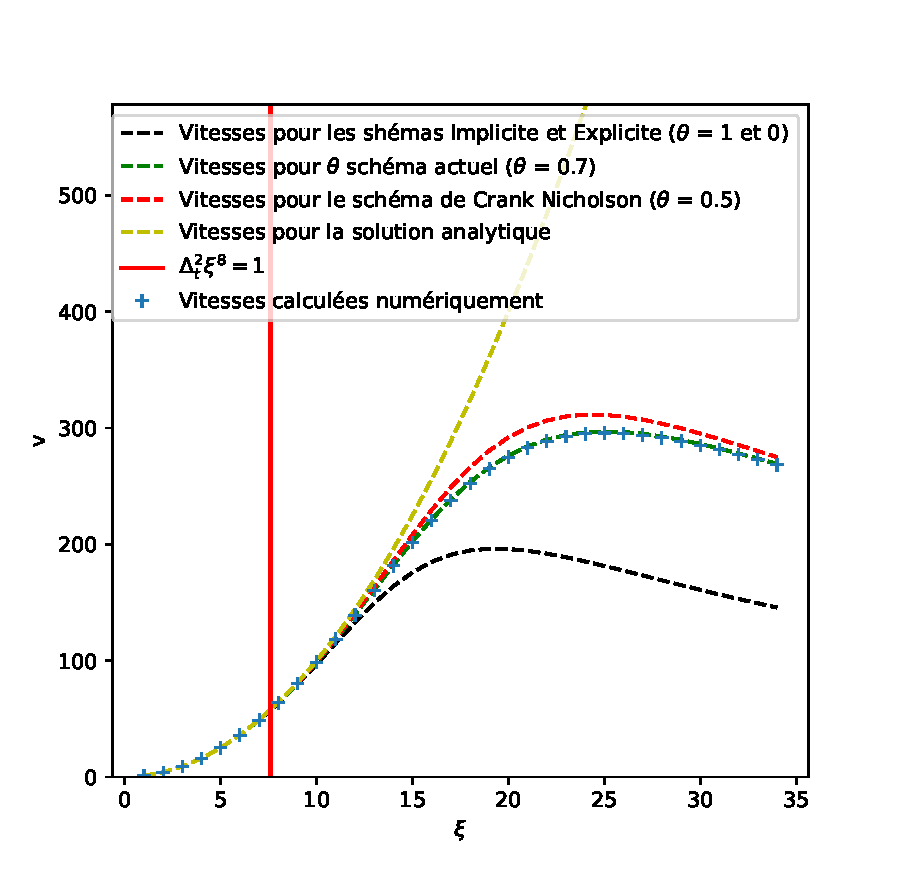
\includegraphics[scale = 0.5]{graphs/v_xi en fonction de dt.pdf}
    \caption{Vitesse des harmoniques en fonction de la fréquence pour $\Delta_t = 3\times10^{-4}$}
    \label{fig:enter-label}
\end{figure}

\subsection{Etude numérique de l'équation de KdV}
\subsubsection{Schéma numérique}
\subsubsection{Les solitons}

\end{document}
\paragraph{Exemple :} Après ces changements de variables, (\ref{eq_B2}) devient $$\partial_{z'z'}\phi' + \mu \partial_{x_1' x_1'}\phi'  = 0 ~~~ \text{si }\textbf{X} = \mathbb{R} $$
$$\partial_{z'z'}\phi' + \mu \partial_{x_1'x_1'}\phi' + \mu \gamma^2 \partial_{x_2'x_2'}\phi' = 0 ~~~ \text{si }\textbf{X} = \mathbb{R}^2$$